\subsection{Speech Recognition With Deep Recurrent Neural Networks \cite{Graves2013Speech}}

End-to-end training methods such as \emph{Connectionist Temporal Classification (CTC)} make it possible to train RNNs for sequence labelling problems where the input-output alignment is unknown. However, RNN performance in speech recognition has so far been disappointing. This paper investigates deep recurrent neural networks on the ASR task, and shows that the method achieves a test set error of 17.7\% on the TIMIT phoneme recognition benchmark, which is the best recorded score.

The goal of this paper is to investigate whether RNNs could benefit from depth in space - that is, stacking multiple recurrent hidden layers on top of each other.

\begin{figure}[htbp]
  \centering
  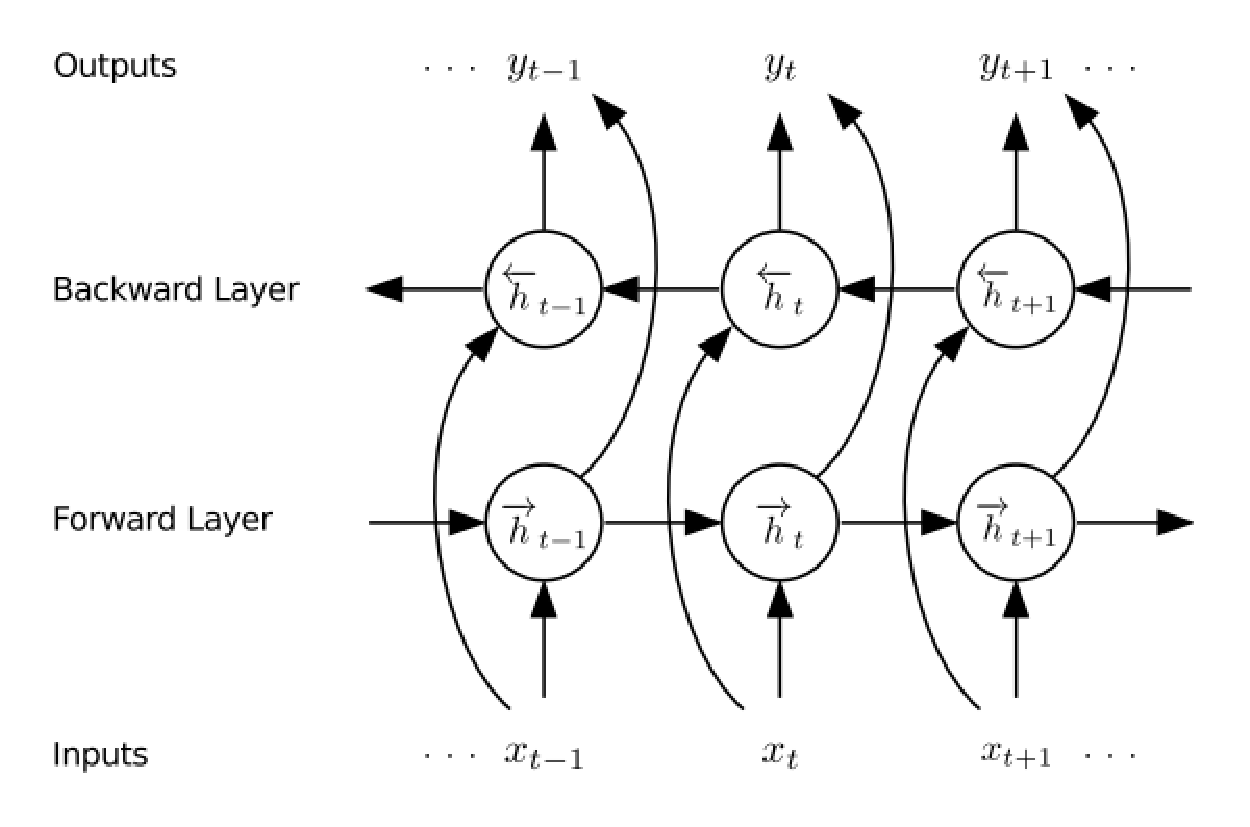
\includegraphics[width=.5\linewidth]{10_17_ASR_RNN}\\
  \caption{Bidirectional RNN}\label{fig:ASR_RNN}
\end{figure}

The concepts of RNN and \emph{long short-term memory (LSTM)} unit have been discussed in previous paper summaries. The basic architecture in this paper is based on the \emph{bidirectional RNNs (BRNNs)}. The basic idea of BRNN is to process the data in both directions (forward and backward) with two separate hidden layers. Figure \ref{fig:ASR_RNN} shows an example of a BRNN model that computes the forward hidden sequence $\stackrel{\rightarrow}{h}$, the backward hidden sequence $\stackrel{\leftarrow}{h}$, and the output sequence $y$. Combining BRNNs with LSTM gives \emph{bidirectional LSTM}.

In the RNN training, the RNNs map directly from acoustic to phonetic sequences. The paper presents two ways to define the output distribution and hence train the network.

The first method is called Connectionist Temporal Classification, which uses a softmax layer to define a separate output distribution $Pr(k|t)$ at every step $t$ along the input sequence. CTC then uses a \emph{forward-backward algorithm} to sum over all possible alignments and determine the normalised probability $Pr(z|x)$ of the target sequence.

The second method is based on the \emph{RNN transducer} technique, which combines a CTC-like network with a separate RNN that predicts each phoneme given the previous ones, thereby yielding a jointly trained acoustic and language model. The basic idea of RNN transducer is to determine a separate distribution $Pr(k | t, u)$ for every combination of input timestep $t$ and output timestep $u$. Specifically, $Pr(k | t, u)$ is defined by taking an `acoustic' distribution $Pr(k | t)$ from the CTC network, a `linguistic' distribution $Pr(k | u)$ from the prediction network, then multiplying them together and renormalising.

In the experimental study, the proposed model is evaluated on the TIMIT corpus. It is reported that the \emph{phoneme error rate (PER)} on the core test set is 17.7\%, which is the best result known to the authors.

Remark: I have also consider the possibility of applying RNNs on the ASR task. This paper shows that this is indeed a promising approach. Compared to the HMM-based or hybrid methods, the approach of this paper is simpler and more elegant - it can jointly train the acoustic and language models in an end-to-end fashion. However, this method is still not very mature, since the TIMIT benchmark is restricted in size. As mentioned by the authors, a possible future work is to extend the system to large vocabulary speech recognition. 